\chapter{Implementation} \label{examplegame}

The final version of Chesskell enables us to describe games of chess, move-by-move. For example, we express a simple 3-move checkmate by the White team as follows:

\begin{lstlisting}
game = chess
    p e4 p f5
    q f3 p g5
    q h5
end
\end{lstlisting}

Note that the spacing is purely for style reasons; the above game could also be written as:

\begin{lstlisting}
game = chess p e4 p f5 q f3 p g5 q h5 end
\end{lstlisting}

\begin{figure}
    \centering
    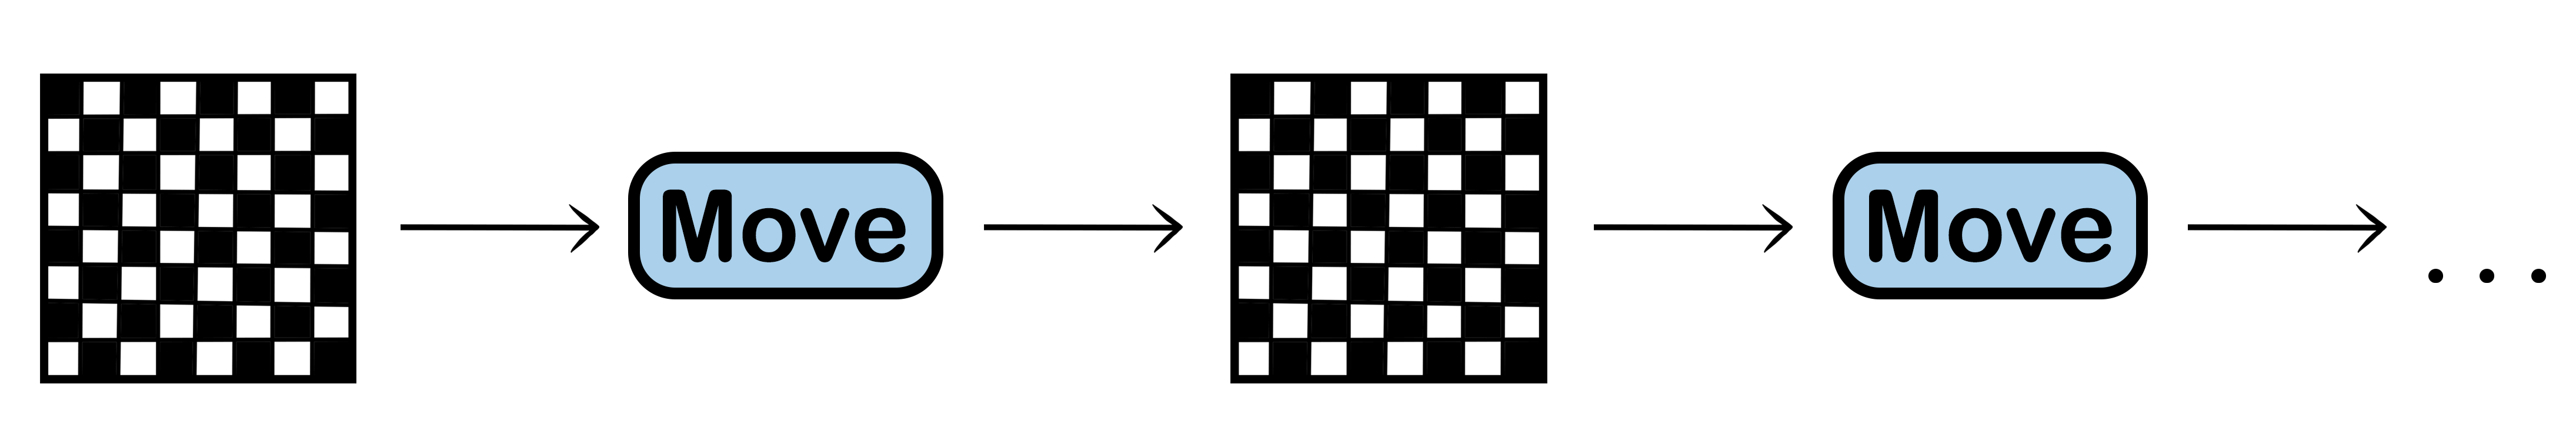
\includegraphics[width=\textwidth,keepaspectratio]{Movefigure.png}
    \caption{A figure demonstrating the chaining of \inline{Move} calls, with each output \inline{BoardDecorator} passed into the next call.}
    \label{movefigure}
\end{figure}

Each move in the Chess game is described with a type family, which takes as input the current state of the board, and outputs the board after the move has been processed (in line with the approach we describe in \cref{chesswithfunctions}). The core movement First Class Family, aptly named \inline{Move}, takes in the position to move from, the position to move to, and the current state of the board, using this information to return a new board state in which the move has been made. Additionally, it updates relevant piece information for the pieces that have moved, which we further detail in this chapter. We give a graphical representation of the process in \cref{movefigure}, and the First Class Family data type for \inline{Move} below:

\begin{lstlisting}
data Move :: Position -> Position -> BoardDecorator -> Exp BoardDecorator
\end{lstlisting}

The EDSL, as we explain in more detail below, uses this \inline{Move} function to perform type-level rule checking of the described Chess game. While the continuation-passing style (CPS) structure complicates the relevant types, the intuition of the EDSL is to take in the current board state, as well as the positions to move from and to, and output the new board state generated by that move. A simplified non-CPS example is below, to aid understanding:

\begin{lstlisting}
edslMove :: Proxy (from :: Position)
         -> Proxy (to :: Position)
         -> Proxy (b :: Board)
         -> Proxy (Eval (Move from to b))
edslMove (x :: Proxy from) (y :: Proxy to) (z :: Proxy (b :: Board))
    = Proxy @(Eval (Move from to b))
\end{lstlisting}

\section{First Class Family Prelude}

In \cref{fcfbackground}, we detail how First Class Families can be utilised to mimic common value-level functions at the type level. While developing Chesskell, we implemented many customary type classes in a First Class Family manner, enabling the final code to be closer to idiomatic Haskell than initially expected.

As an example, consider the \inline{Foldable} typeclass\footnote{\url{https://hackage.haskell.org/package/base-4.15.0.0/docs/Data-Foldable.html}}, which enables value-level data structures with defined \inline{foldr} or \inline{foldMap} instances to be used with many functions written for \inline{Foldable} structures. The type for \inline{foldr} is as follows:

\begin{lstlisting}
foldr :: Foldable t => (a -> b -> b) -> b -> t a -> b
\end{lstlisting}

A value-level function to compute the sum of entries in any foldable collection of integers could be written as such, allowing this definition to be used with any value of a type which implements \inline{Foldable}:

\begin{lstlisting}
sum :: Foldable f => f Int -> Int
sum xs = foldr (+) 0 xs
\end{lstlisting}

In Chesskell, we can express similar behaviour through the use of a new data type, \inline{Foldr}, which we give below with an \inline{Eval} instance for lists:

\begin{lstlisting}
data Foldr :: (a -> b -> Exp b) -> b -> f a -> Exp b
type instance Eval (Foldr f z '[])       = z
type instance Eval (Foldr f z (x ': xs))
    = Eval (f x (Eval (Foldr f z xs)))
\end{lstlisting}

Now, type-level versions of common \inline{Foldable} functions, such as \inline{sum} and \inline{length}, can be implemented using this definition of \inline{Foldr}. We give a type-level First Class Family definition of \inline{Sum} below, along with a simple First Class Family version of natural number addition:

\begin{lstlisting}
data Sum :: f Nat -> Nat
type instance Eval (Sum xs) = Foldr (:+) Z xs

data (:+) :: Nat -> Nat -> Exp Nat
type instance Eval (x :+ y) = x + y
\end{lstlisting}

Mimicking type classes in this manner allows us to implement behaviour akin to Monads and Applicative Functors~\cite{applicatives}. There are certain rules in Chess that would require excessive amounts of pattern-matching to express with closed type families, prompting this effort. In addition to Foldr, Chesskell also includes First Class Family versions of FMap \inline{(<\$>)}, Apply \inline{<*>}, and Bind \inline{(>>=)} (among others), to enable Functor, Applicative Functor, and Monadic behaviour at the type level. We give the definitions of \inline{Bind} and \inline{(>>=)} below, with an \inline{Eval} instance for \inline{Maybe} types, to illustrate:

\begin{lstlisting}
data Bind :: m a -> (a -> Exp (m b)) -> Exp (m b)
type instance Eval (Bind Nothing  f)  = Nothing
type instance Eval (Bind (Just x) f)  = Eval (f x)

data (>>=) :: m a -> (a -> Exp (m b)) -> Exp (m b)
type instance Eval (x >>= f) = Eval (Bind x f)
\end{lstlisting}

\section{Type-Level Chess}

The Chesskell library includes a full representation of a game of Chess at the type-level, as we explain below. The model is checked move-by-move, with the current board state (as well as some additional information) carried between moves via a \inline{BoardDecorator} type. This \inline{BoardDecorator} contains all information necessary to encapsulate the current state of a game of chess; in other words, Chesskell does not rely on any global state, and the game state itself is easily modifiable (enabling the development of board creation syntax, which we detail in \cref{boardcreation}).

\subsection{Chess Types and Kinds}

This section details the types involved, including the board representation; we describe Chesskell's types from the bottom up, since the types here are composite and require understanding of other types.

\subsubsection{Team and PieceName}

Both \inline{Team} and \inline{PieceName} are simple algebraic data types, with all constructors defined in code. The \inline{Team} type enumerates all teams a piece can belong to; \inline{Black} and \inline{White}. The \inline{PieceName} type enumerates all possible names of pieces; Pawn, Rook, and so on. Thanks to promotion, as we explain in \cref{promotionsection}, these types are immediately available for use with Type Families.

\begin{lstlisting}
data Team = Black | White
data PieceName = Pawn
               | Bishop
               | Knight
               | Rook
               | King
               | Queen
\end{lstlisting}

\subsubsection{Position}

The \inline{Position} type holds the positions of pieces on the chess board. It makes use of two more types; one for columns and the other for rows (we explain details on columns and rows in \cref{boarddetails}). The \inline{Column} type is another simple algebraic data type enumerating all columns that a piece can reside within. The row type is a type-level implementation of Peano natural numbers, named \inline{Nat}. Early versions of Chesskell had a custom implementation, but the final version uses definitions provided in \inline{Data.Type.Nat}. We give a definition of \inline{Nat} below, for understanding:

\begin{lstlisting}
data Column = A | B | C | D | E | F | G | H
data Nat where
    Z :: Nat
    S :: Nat -> Nat
\end{lstlisting}

Note that the \inline{Position} kind has a potentially infinite number of valid types, but only 64 of these types are valid chess positions. As such, we define an associated type family, \inline{IsValidPosition}, which outputs \inline{True} if the given position is a valid chess position, and \inline{False} otherwise. We give the definition of the \inline{Position} type below:

\begin{lstlisting}
data Position where
    At :: Column -> Nat -> Position
\end{lstlisting}

\subsubsection{The Pieces}

Each piece, represented by the \inline{Piece} type, contains information relevant for rule checking: that piece's team, name, and an information type. The information type, named \inline{PieceInfo}, contains a \inline{Nat} and a \inline{Position}, to represent the number of moves that piece has taken, and its current position on the board (respectively). Recording the number of moves the piece has taken is important for several rules in chess, including castling and \textit{en passant} capture (as we discuss in \cref{castlesection,passantsection}), and so is included in the \inline{PieceInfo} type.

The \inline{PieceInfo} type was created separately from the plain \inline{Piece} type so that if any further information was required, it could be added without breaking existing \inline{Piece} pattern-match definitions.

\begin{lstlisting}
data PieceInfo where
    Info :: Nat -> Position -> PieceInfo

data Piece where
    MkPiece :: Team -> PieceName -> PieceInfo -> Piece
\end{lstlisting}

There are several utility Type Families defined for the \inline{PieceInfo} type to simplify code; such as \inline{GetPosition}, a First Class Family which gets the position information from a given \inline{PieceInfo} type.

\subsubsection{The Board} \label{boardtypesection}

We explain in \cref{lengthindexedvectors} that length-indexed vectors are an ideal choice for representing the Chess board, as Chess boards have a fixed constant size; with length-indexed vectors, we can enforce the length of the vector in its type, ensuring that the Chess board does not change size. Therefore, it is appropriate to express the board as a vector of 8 vectors of 8 \inline{Maybe Piece}-s. We use \inline{Maybe Piece} instead of just \inline{Piece} because a board square does not necessarily contain a piece:

\begin{lstlisting}
type Eight = (S (S (S (S (S (S (S (S Z))))))))
type Row   = Vec Eight (Maybe Piece)
type Board = Vec Eight Row
\end{lstlisting}

Although this is the main board type, it is augmented with a \inline{BoardDecorator}, so named because the intention is similar to the decorator design pattern~\cite{decorator}, with the exception that sub-classing and super-classing are not features of Haskell. In most cases, we use \inline{BoardDecorator} instead of \inline{Board}, since it contains additional information:

\begin{itemize}
    \item The last team to move;
    \item The last position moved to;
    \item The White and Black King positions, stored as a tuple;
    \item The number of moves in the game thus far.
\end{itemize}

Previous versions of the program, to find the King positions (for the frequent operation of determining if either King is in check), would pass repeatedly over the \inline{Board}. Having their positions available in the decorator avoids the performance cost of making these passes. While this approach introduces overhead (the \inline{BoardDecorator} must be updated each move), the code is much conceptually clearer with the use of the decorator. We give the definition of \inline{BoardDecorator} below:

\begin{lstlisting}
data BoardDecorator where
    Dec :: Board
        -> Team
        -> Position
        -> (Position, Position)
        -> Nat
        -> BoardDecorator
\end{lstlisting}

\subsection{Custom Type Errors}

In Chesskell, we use definitions found in \inline{GHC.TypeLits} to express custom type errors. These definitions include a type family, \inline{TypeError}, and a data type \inline{ErrorMessage}, to enable programmers to generate type errors with arbitrary error messages. For instance, the type below (when type-checked) will cause GHC to halt compilation and generate a type error:

\begin{lstlisting}
type ErrTest = TypeError (Text "Custom error!")
\end{lstlisting}

As expected, the generated type error matches the input \inline{ErrorMessage} argument:

\begin{lstlisting}
-- Below results in the following type error:
    -- * Custom error!
    -- * In the type synonym declaration for 'ErrTest'
type ErrTest = TypeError (Text "Custom error!")
\end{lstlisting}

In GHC, the kind returned by \inline{TypeError} is polymorphic; and so the output of a \inline{TypeError} application can be returned from type families with no issues. The book Thinking With Types~\cite{twt} contains a First Class Family equivalent definition, named \inline{TE'}:

\begin{lstlisting}
data TE' :: ErrorMessage -> Exp a
type instance Eval (TE' msg) = TypeError msg
\end{lstlisting}

In Chesskell, we use this definition to return a type error in circumstances where an \inline{Exp a} type is expected (for some type \inline{a}). To illustrate, consider the below definition:

\begin{lstlisting}
type TETest = Eval (If ('True)
    ('Just 5) -- then
    (TE' (Text "Some error"))) -- else
\end{lstlisting}

Assuming that the \inline{If} First Class Family behaves similarly to if-then-else expressions in Haskell, we expect \inline{TETest} to unify with \inline{'Just 5}. This is the case --- it compiles successfully. However, if we pass in a \inline{'False} type instead of a \inline{'True} type as the if condition, the custom type error is thrown:

\begin{lstlisting}
-- Below results in the following type error:
    -- * Some error
    -- * In the type synonym declaration for 'TETest'
type TETest = Eval (If ('False)
    ('Just 5) -- then
    (TE' (Text "Some error"))) -- else
\end{lstlisting}

\subsection{Chess Rules}

In Chesskell, the rules of Chess are expressed as First Class Families that either return a \inline{BoardDecorator} or a type error (as we explain in \cref{chessrules}). Each such rule-check type family has the suffix \inline{-Check}, such as the aptly named \inline{NotTakingKingCheck} and \inline{NotTakingOwnTeamCheck}. These checks are broadly split into pre-move checks, and post-move checks; each check includes a custom error message to make clear to the user where exactly the rule violation occurs.

To illustrate, we give the definition of \inline{NotSamePosCheck}, which checks that the described move is between two distinct positions, and generates a type error otherwise:

\begin{lstlisting}
data NotSamePosCheck :: Position -> Position -> BoardDecorator -> Exp BoardDecorator
type instance Eval (NotSamePosCheck fromPos toPos boardDec)
    = If' (Eval (fromPos :==: toPos))
        (TE' (TL.Text ("Moves from a position to that same position are not allowed.")))
        (ID boardDec)
\end{lstlisting}

We combine and compose rule checks with a First Class Family version of the function composition operator, \inline{(.)}:

\begin{lstlisting}
NotSamePosCheck . ExampleCheck1 . ExampleCheck2
\end{lstlisting}

\subsubsection{Movement Rules}

Each piece's movement is subject to a specific set of rules for that piece. For instance, a King can move a single space in any direction. The \inline{PieceMoveList} First Class Family formalises this, returning a list of spaces that a piece can move to, given that piece as a \inline{Piece} type, and a \inline{BoardDecorator} representing the current state of the board.

\begin{lstlisting}
data PieceMoveList :: Piece -> BoardDecorator -> Exp [Position]
\end{lstlisting}

Consider a \inline{PieceMoveList} instance for Bishops:

\begin{lstlisting}
type instance Eval (PieceMoveList (MkPiece team Bishop info) boardDec)
    = Eval (AllReachableDiag team boardDec (Eval (GetPosition info)))
\end{lstlisting}

Bishops can move diagonally in a straight line by any number of spaces. The type family \inline{AllReachableDiag} is used to get a list of all diagonally ``reachable'' positions. It takes in the \inline{Position} of the relevant piece, that piece's \inline{Team}, and the current state of the board as a \inline{BoardDecorator}. It outputs all diagonal positions that piece can move to.

Reachability for a given direction is defined in Chesskell as all the empty spaces in that direction, stopping at either the first occupied space or the edge of the board. That space is included or excluded depending on whether that space is occupied by a piece of the opposite team, since an attacking piece could move to that space and take the piece there.

We ensure correctness of movement with a pre-move rule-check, named \inline{CanMoveCheck} with kind \inline{Position -> Position -> BoardDecorator -> Exp BoardDecorator}, which checks if there is a piece at the first position that can move to the second position. Additionally, for more specific error messages, there exist a few additional checks, such as \inline{TeamCheck}, which ensures that the same team does not move twice in a row.

The move list, in most cases, prunes all invalid moves for that piece so that any position in the move list for that piece is a valid movement destination. However, there is one important exception: King movement. The move list for a King can include invalid King movement positions, as the move list generation does not check that the King does not move into the attack path of other pieces (i.e. that it doesn't move into check).

This is deliberate, since check is determined on a position-by-position basis, and checking 8 potential positions for check would be expensive. Instead, we make use of a post-move rule-check named \inline{CheckNoCheck} (which we detail in \cref{checksection}) to ensure that neither King moves into check.

\subsubsection{Attack/Capture Rules}

Although they are similar, the list of spaces that a piece can attack and the list of spaces that a piece can move to are not the same. It is neither true that every position a piece can attack is one that it can move to, nor that every position that can be moved to is under attack; for example, pieces can attack the King of the opposite team, but cannot directly move to that King's position and capture it. There are other differences as well, most notably for Pawns and Kings; so \inline{PieceMoveList} cannot be used in general to determine which squares a piece can attack. To address these shortcomings, we define another type family, \inline{PieceAttackList}, which gives the list of all squares that a piece can attack.

\paragraph{Checking for Check} \label{checksection}

One of the most important rules in Chess, that of placing the opposite King in check, cannot be expressed solely through move and attack lists. Any movement can place either King in check, and it is not always the case that a movement by a piece places the opposite King in check; a move may be ruled as invalid because it places that piece's King into check. For instance, if a Black Rook stands between a White Queen and a Black King, the Rook is not allowed to move out of the Queen's attack path, since such a move would put the Black King into check.

However, the only time that check is relevant is after each move. A move by a piece is invalid when it places that piece's King in check, or if it leaves that piece's King in check. We can express this rule with a post-move check, implemented as a First Class Family \inline{CheckNoCheck}.

Early versions of Chesskell naively computed and combined all attack lists for all pieces, and simply checked if the King's position was a member of that combined list. A more efficient approach, found in Chesskell today, is to emulate other pieces' movement code from the King's position.

This approach is based off of the observation that for all pieces except Kings and Pawns, if they can move from position a to position b, then they can also move from b to a. As an illustration, if a Queen at the King's position (of the same team as the King) would be able to reach a Queen of the opposite team, then the King would be in check.

We leverage this behaviour to detect when a King is in check. Several ``rays'' are sent out from the King's position in horizontal, vertical, and diagonal directions (8 in total). These rays detect Queens of the opposite team, as well as Bishops (for diagonal rays) and Rooks (for horizontal and vertical rays). Attacking Pawns are also checked here, for the immediate diagonal positions either above the King (if the King is White) or below the King. If the ray reaches an attacking piece, the ray function returns true; otherwise, it returns false. The ray will immediately stop being cast, and report back with no check possible in that direction (i.e. a \inline{False} type), if a piece of the same team as the King is encountered (since they would block the attack path of a piece of the opposite team).

In addition to the ray approach, we apply Knight movement rules (from the King's position) to check if there are any Knights that could reach the King and place them in check.

There is one last piece type not handled by the above method---Kings. This is deliberate; it would be illegal for a King to move within attacking distance of the opposite King, since then the moving King would be in check.

A code snippet for determining if the King is in check, which checks if any of the above conditions are true, is below for understanding. The First Class Family \inline{Any} returns true if any elements of a list of Booleans are true, and false otherwise. Each of the -\inline{Ray} functions returns true if a piece could place a King in check from that direction, and the \inline{IsKnightAttacking} function returns true if any Knights of the opposite team are reachable from the given position:

\begin{lstlisting}
data IsKingInCheck :: Position
                   -> Team
                   -> BoardDecorator
                   -> Exp Bool
type instance Eval (IsKingInCheck kingPos team boardDec)
    = Eval (Any '[
    SendLeftRay kingPos team boardDec,
    SendRightRay kingPos team boardDec,
    -- ...
    -- Send rays above, below, and in all 4 diagonal directions
    -- ...
    IsKnightAttacking kingPos team boardDec ])
\end{lstlisting}

\subsubsection{Exceptional Rules}

There are a few Chess rules that are dissimilar from all other Chess rules; and implementing these rules requires a different approach from other rule implementations. Since they are of particular interest, the implementation of these rules is detailed here.

\paragraph{Castling} \label{castlesection}

Most Chess rules move a single piece, and can capture another piece to remove it from play. However, the \emph{Castling} move involves the movement of two pieces; the King, and one of their Rooks. Castling can only occur if neither the King nor the Rooks have moved, as long as none of the positions the King would move through are under check, and there are no other pieces between the King and the Rook. It is one of the most complex rules of Chess, and requires many tests before it can proceed.

There are two varieties of Castle; Queen-side Castle and King-side Castle, depending on the direction that the King moves in (either left or right, respectively). Both varieties are shown for the White team in \cref{queensidecastle,kingsidecastle}. Essentially, the King moves either 2 or 3 spaces towards the Rook, and the Rook wraps around to the other side of the King.

In Chesskell, we model castling as a move by the King; valid castling positions are added to the King's move list. A type family, \inline{CanCastle}, is responsible for checking if the King of a certain team can indeed perform castling in either direction, returning a pair of Booleans to state whether the King can castle left or right. The below code snippet illustrates a part of this process:

\begin{lstlisting}
type family CanCastle (t :: Team) (b :: BoardDecorator) :: (Bool, Bool) where
    CanCastle team boardDec = If' (Not' (HasKingMoved team boardDec))
        (ID (CanCastleToEitherRook team boardDec))
        (ID '(False, False))
\end{lstlisting}

The above code first checks if the King has moved; if they have not, then it checks if both Rooks have not moved. If they have not moved either, then it determines if any of the spaces the King would move through are in check, and then if there are any pieces between the King and the Rook. This logical AND chaining is performed using a type family \inline{PairAnd}, which performs element-wise logical AND on ordered pairs of Boolean types.

These checks must pass for the King to be able to castle in that direction; and a pair of Booleans is returned signifying if the King can castle in either direction. For instance, if the King can castle left but not right, then \inline{CanCastle} will return \inline{'(True, False)}.

This extended Castling check illustrates why it is useful to have each piece's move count in the \inline{PieceInfo} type; it enables quickly determining if a King or either of the Rooks have moved. Simply checking if the King or Rooks are in their starting positions is not enough, since they could have just moved back to those positions.

There are no circumstances under which a King is obligated to castle, and so there are no pre- or post-move rule checks. However, a King cannot castle to capture another piece; so these castle positions are not a part of the King's attack list.

\begin{figure}[h]
    \centering
    \fenboard{8/8/8/8/8/8/8/R3K3 w KQkq - 0 1}
    \showboard
    \hidemoves{1. O-O-O}
    \quad
    \showboard
    \caption{A pair of figures, showing a Queen-side Castle involving the White King.}
    \label{queensidecastle}
\end{figure}

\begin{figure}[h]
    \centering
    \fenboard{8/8/8/8/8/8/8/4K2R w KQkq - 0 1}
    \showboard
    \hidemoves{1. O-O}
    \quad
    \showboard
    \caption{A pair of figures, showing a King-side Castle involving the White King.}
    \label{kingsidecastle}
\end{figure}

\paragraph{Pawn Movement and En Passant} \label{passantsection}

Pawns have the most complex movement rules out of any piece, primarily because their attack patterns are different from their movement patterns. Pawns can move one vertical space forwards, but on their first move can move two spaces instead of one. (For a White Pawn, ``forwards'' means towards a row of higher number, and for a Black Pawn, it means towards a row of lower number --- see \cref{pawnfirstmovement}.) However, they cannot capture a piece this way; they can only capture one diagonal space in front of themselves.

\begin{figure}
    \centering
    \fenboard{8/2p5/8/8/8/8/5P2/8 w - - 0 1}
    \chessboard[showmover=false, pgfstyle=cross, color=black, linewidth=0.15em, shortenstart=0.5ex, shortenend=0.5ex, markfields={c5,c6,f3,f4}]
    \caption{A figure demonstrating the positions that a Black and a White Pawn can move to on their first movement.}
    \label{pawnfirstmovement}
\end{figure}

This means that a Pawn can indeed make a diagonal move, but only if there is a capturable piece there. (For instance, a Black Pawn could move downwards diagonally by a single space to capture a White Bishop, but could not move to that square if it were empty or if it were occupied by a White King.) Additionally, Pawns have one more special capture rule; that of \emph{en passant}.

A Pawn can perform an \emph{en passant} capture if a Pawn of the opposite team has moved forwards by two spaces last turn (which can only occur if that was the opposite Pawn's first move), and ended up next to the attacking Pawn. In this situation, the original attacking Pawn can move diagonally to the empty space behind the opposite team's Pawn, capturing it. See \cref{enpassantfigure} for a graphical representation, showing a White Pawn performing \emph{en passant} capture on a Black Pawn.

\begin{figure}
    \centering
    \fenboard{8/2p5/8/3P4/8/8/8/8 b - - 0 1}
    \scalebox{0.7}{\chessboard[showmover=false, pgfstyle=straightmove, arrow=to, linewidth=0.1em, shortenstart=0.5ex, markmoves={c7-c5}]}
    \hidemoves{1... c5}
    \scalebox{0.7}{\chessboard[showmover=false, pgfstyle=straightmove, arrow=to, linewidth=0.1em, shortenstart=0.5ex, markmoves={d5-c6}]}
    \fenboard{8/8/2P5/8/8/8/8/8 b - - 0 1}
    \scalebox{0.7}{\chessboard[showmover=false]}
    \caption{A sequence of three Chess boards, demonstrating an \emph{en passant} capture by White of a Black Pawn.}
    \label{enpassantfigure}
\end{figure}

This capture rule is dependent on several factors; the last move made, as well as the relative positions of the pieces. Furthermore, the capture move does not result in the attacking piece landing on the square of the piece being captured; making it distinct from all other capture rules.

We define a type family, \inline{GetEnPassantPosition}, which is responsible for determining if an \emph{en passant} capture is a valid move for a pawn at a given position:

\begin{lstlisting}
data GetEnPassantPosition :: Position
                          -> BoardDecorator
                          -> Exp [Position]
type instance Eval (GetEnPassantPosition pos boardDec)
    = If'
        (Eval ((GetLastPosition boardDec) `In` Eval (GetLeftRightPositions pos)))  -- condition
    (FromMaybe '[] (EnPassantPosition (GetMovingTeam boardDec) . PiecePosition)
        (Eval (GetPieceAtWhichDec boardDec (GetLastPosition boardDec) (IsPawn .&. PawnMovedTwoLast))))  -- then
        (ID '[])  --else
\end{lstlisting}

First, the type family checks if the position moved to last turn (fetched from the \inline{BoardDecorator} with \inline{GetLastPosition}) is either to the left or the right of the given pawn position. This is the check to determine whether any piece just moved to the left or right of the current Pawn. If this check passes, then there is another check; whether the piece that made that move was a Pawn, and whether it moved two spaces. If that check passes, then the piece's position is fetched and the row is either incremented or decremented (depending on the attacking team) by the type family \inline{EnPassantPosition} to get the single space either above or below that piece --- the target square to perform \emph{en passant} capture.

We use First Class Families to simplify these logical checks. \inline{GetPieceAtWhichDec} returns a \inline{Maybe Piece} depending on whether there is a piece at a given position which fulfils a given predicate, returning \inline{Nothing} if the predicate does not evaluate to true, and the \inline{Just}-wrapped piece otherwise. Additionally, a type-level First Class Family version of \inline{FromMaybe} is used to either transform the \inline{Nothing} type into an empty list \inline{'[]}, or to transform the wrapped value into a singleton list containing the \emph{en passant} capture position.

Implementing \emph{en passant} captures was the driving factor that prompted the creation of the \inline{BoardDecorator} type, since the last position moved to was required as part of the process. Ultimately, \emph{en passant} captures are implemented in Chesskell, as we demonstrate with the successful compilation of the below game:

\begin{lstlisting}
enPassant = chess
    p d4 p a6
    p d5 p e5
    p e6  -- En Passant capture!
end
\end{lstlisting}

\paragraph{Pawn Promotion}

Pawns have one last complex movement rule; that of promotion. When a Pawn makes it to the opposite side of the Board, they must be promoted to another piece type; either a Queen, a Bishop, a Rook, or a Knight. Pawns must be promoted; they cannot opt out of promotion.

Implementing Pawn promotion proved difficult, since the core \inline{Move} family we describe in \cref{examplegame} does not hold enough information to determine what piece type a Pawn should be promoted to. While one potential solution is to hold this information as a \inline{Maybe PieceName} in the \inline{BoardDecorator}, promotion is infrequent and never occurs in many games. Therefore, instead of using the base \inline{Move} First Class Family, we define a new First Class Family called \inline{PromotePawnMove} to be used when promotion is necessary:

\enlargethispage{\baselineskip}  % Avoid widow in listing below

\begin{lstlisting}
data PromotePawnMove :: Position -> Position -> PieceName -> BoardDecorator -> Exp BoardDecorator
type instance Eval (PromotePawnMove fromPos toPos promoteTo boardDec)
    = If' (Eval (IsPieceAtWhichDec boardDec fromPos (IsPiece Pawn)))
        ((PromotePieceTo promoteTo toPos . Move fromPos toPos) boardDec)
        (If (Eval (IsPieceAt boardDec fromPos))
            (TE' (TL.Text ("The piece at: " ++ TypeShow fromPos ++ " is not a " ++ TypeShow Pawn ++ ". Non-Pawn pieces cannot be promoted.")))
            (TE' (TL.Text ("There is no piece at: " ++ TypeShow fromPos ++ "."))))
\end{lstlisting}

\inline{PromotePawnMove} is similar to \inline{Move}, and indeed calls it internally; but in addition to promoting the piece after it has moved, it ensures that the position to be moved from contains a Pawn (since it is the only piece type that can be promoted).

The type family \inline{PromotePieceTo} of kind \inline{PieceName -> Position -> BoardDecorator -> Exp BoardDecorator} is responsible for changing the \inline{PieceName} of the Pawn piece once it has reached the opposite end of the board. It applies a First Class Family, \inline{PromoteTo}, to the piece at the given position to change its \inline{PieceName} to some given one. Additionally, it generates a type error if the user attempts to promote the Pawn to a King or another Pawn.

However, \inline{PromotePieceTo} and \inline{PromotePawnMove} alone are not enough; because a Pawn must always promote when it reaches the opposite end of the board. To enforce this rule, we define a post-move check named \inline{ShouldHavePromotedCheck}, which is responsible for determining whether a promotion should have occurred at the last move or not. The First Class Family definition simply calls a type family:

\begin{lstlisting}
data ShouldHavePromotedCheck :: Position -> BoardDecorator -> Exp BoardDecorator
type instance Eval (ShouldHavePromotedCheck toPos boardDec)
    = ShouldHavePromotedCheck' toPos boardDec
\end{lstlisting}

The \inline{ShouldHavePromotedCheck'} type family takes in the last position moved to, and the post-movement \inline{BoardDecorator}. If the last move was to the top or bottom rows (i.e. the 8th or the 1st), it checks if there is a Pawn at that position. If so, it generates a type error (since such a Pawn should have been promoted). Otherwise, it returns the input \inline{BoardDecorator}. We give part of the definition below, to illustrate:

\begin{lstlisting}
type family ShouldHavePromotedCheck' (t :: Position) (b :: BoardDecorator) :: BoardDecorator where
    -- ...
    ShouldHavePromotedCheck' (At col Nat8) boardDec
        = If'
            (Eval (IsPieceAtWhichDec boardDec (At col Nat8) (IsPawn .&. HasTeam White))) -- condition
                (TE' (TL.Text ("Promotion should have occurred at: " ++ TypeShow (At col Nat8) ++ ". Pawns must be promoted when they reach the opposite end of the board.")))  -- then
            (ID boardDec) -- else
    -- ...
\end{lstlisting}

Pawn promotion is successfully implemented in Chesskell --- if a pawn should fail to promote during a game of Chess, then a descriptive type error is generated:

\begin{lstlisting}
-- Below results in the following type error:
-- error: Promotion should have occurred at: A8. Pawns must be promoted when they reach the opposite end of the board.
failedToPromote = create
    put _Wh _P at a7
startMoves
    p a8
end
\end{lstlisting}

\section{The EDSL}

The EDSL has gone through multiple changes during development, not only in syntax but also in feature set. This section of the dissertation details the changes the Chesskell EDSL has undergone, explaining the design decisions along the way.

\subsection{Minimum Viable Product}

Before the final format and syntax of the EDSL was decided upon, it was important to determine whether the creation of a value-level interface for the type level model was possible at all. The earliest version of the ``EDSL'' was a set of named Haskell functions, to test if the type-level model was usable by value-level functions.

This Minimum Viable Product version does not include any of the more advanced features of the final EDSLs (such as board creation), but successfully allows the user to describe a Chess game move by move. A single core function, named \inline{move}, made use of \inline{Proxy} types and a First Class Family version of bind to move a piece on a board from one position to another:

\begin{lstlisting}
move :: Proxy (from :: Position)
     -> Proxy (to :: Position)
     -> Proxy (b :: Maybe Board)
     -> Proxy (Eval (b >>= Move from to))
move (sFrom :: Proxy from) (sTo :: Proxy to) (pBoard :: Proxy (b :: Maybe Board))
    = Proxy @(Eval (b >>= Move from to))
\end{lstlisting}

Despite its simple nature, \inline{move} alone is sufficient for a user to interact with the type-level model of Chess and describe a game. It is a viable and minimal version of Chesskell --- if not much of an EDSL.

\subsection{Flat Builders}

Once the feasibility of a Chesskell EDSL was proven, the actual format and logic of the EDSL was to be decided upon. A Continuation Passing Style scheme (as we briefly outline in \cref{cpsshortexample}) forms the foundation for the EDSL, with inspiration taken from Dmitrij Szamozvancev's Flat Builders pattern~\cite{mezzo}. The core idea is value transformation through a series of continuation function applications, until the final continuation function returns a value.

The type \inline{Spec t} is the type of functions which take in a continuation to operate on a value of type \inline{t}. For instance, a function with type \inline{Int -> Spec Int} would take in an integer, and then a continuation to operate on that integer.

\begin{lstlisting}
type Spec t = forall m. (t -> m) -> m
\end{lstlisting}

A function with type \inline{Int -> Spec Int} can be represented with \inline{Conv Int Int} --- the \inline{Conv s t} type represents functions which convert a value of type \inline{s} to a value of type \inline{Spec t}.

\begin{lstlisting}
type Conv s t = s -> Spec t
\end{lstlisting}

Finally, the \inline{Term t r} type ends the continuation stream by taking no continuations; instead, we pass in a value of type \inline{t}, returning a value of type \inline{r}. If \inline{t} and \inline{r} are equal, then an implementation would match that of \inline{id}, the identity function.

\begin{lstlisting}
type Term t r = t -> r
\end{lstlisting}

As an illustrative example of how we use these types, consider the implementation of a sentence-like structure for mathematical operations, such as \inline{to 5 add 7 add 9 increment _then _print}, which should return a string version of the final result. We can achieve this using the Flat Builders pattern. We define \inline{to} like so, passing a number into a continuation which performs some computation on the input:

\begin{lstlisting}
to :: Int -> Spec Int
to x cont = cont x
\end{lstlisting}

We define \inline{add} to take in two input numbers, adding them together, and passing the result to an input continuation:

\begin{lstlisting}
add :: Int -> Int -> Spec Int
add x y cont = cont (x + y)
\end{lstlisting}

We define \inline{increment} like so:

\begin{lstlisting}
increment :: Int -> Spec Int
increment x cont = cont (x + 1)
\end{lstlisting}

The continuation \inline{_then} is intended purely to clarify operations, not to perform any new computation:

\begin{lstlisting}
_then :: Int -> Spec Int
_then x cont = cont x
\end{lstlisting}

And finally, we define the \inline{_print} continuation, which enables us to end the continuation stream and return a string:

\begin{lstlisting}
_print :: Term Int String
_print x = show x
\end{lstlisting}

Using all of these continuations, we can verify that the sentence-like expression \inline{to 5 add 7 add 9 increment _then _print} is well-typed and returns \inline{"22"}, a string.

Note that none of these continuations make assumptions about the kinds of operations performed within the next continuation; only that they take in an integer. Adding new operations, such as multiplication or division, is as simple as adding a new continuation which performs this operation. Such an approach is a natural fit for Chesskell, since the various Chess moves can be (relatively) encapsulated, and it becomes straightforward to extend the EDSL (such as the extensions we discuss in \cref{castleextension,numberextension}).

We combine these Flat Builders continuation types with type-level rule checks, to create a Chess EDSL that operates through passing continuations. Using a combination of proxies, kind signatures, and type applications, we enforce type-level rule checking upon the value-level EDSL.

\subsection{Chess Continuations}

In this section, we discuss the rationale behind and definitions created for Chesskell's long-form syntax. For details on the shorthand syntax, see \cref{shorthandexplanation}.

The chess game starts with a \inline{Proxy} value, whose \inline{Proxy} type is parameterised with a \inline{BoardDecorator} type (i.e. the value has type \inline{Proxy BoardDecorator}). We apply continuations, transforming that value, until the chess game ends\footnote{Note that users can still express games which break rules; these games are just not well-typed.}. Chess games begin with the board in a set configuration; and so we define a type \inline{StartDec} of kind \inline{BoardDecorator} to contain all of this information.

\begin{lstlisting}
chess :: Spec (Proxy StartDec)
chess cont = cont (Proxy @StartDec)
\end{lstlisting}

Each core continuation is named after a piece type, such as \inline{pawn} or \inline{king}. All take in a \inline{Proxy (a :: Position)}, a \inline{Proxy} value whose type is parameterised with the relevant \inline{Position} type. We define a new data type, \inline{MoveArgs}, in order to simplify the process of passing information between the continuations; while the \inline{Move} family is a First Class Family, and can be partially applied, it takes in no \inline{PieceName} argument, and so cannot contain all the relevant types which must pass between the continuations.

\begin{lstlisting}
data MoveArgs where
    MA :: BoardDecorator
       -> Position
       -> PieceName
       -> Position
       -> MoveArgs
\end{lstlisting}

We give the definition of the \inline{pawn} continuation below as an example; however, all piece continuations are similar, and only differ in the \inline{PieceName} type passed to the continuation via \inline{MoveArgs}.

\begin{lstlisting}
pawn :: Proxy (b :: BoardDecorator)
     -> Proxy (fromPos :: Position)
     -> Spec (Proxy (MA b fromPos 'Pawn))
pawn (dec :: Proxy b) (from :: Proxy fromPos) cont
    = cont (Proxy @(MA b fromPos Pawn))
\end{lstlisting}

The next continuation, \inline{to}, takes in another \inline{Proxy (a :: Position)} as well as the \lstinline{MoveArgs}, performs the move computation, puts the resulting board decorator into a \inline{Proxy} type, and passes that \inline{Proxy} into the continuation given.

\begin{lstlisting}
to :: Proxy (MA (b :: BoardDecorator) (fromPos :: Position) (n :: PieceName))
   -> Proxy (toPos :: Position)
   -> Spec (Proxy (Eval (MoveWithStateCheck n fromPos toPos b)))
to (args :: Proxy (MA (b :: BoardDecorator) (fromPos :: Position) (n :: PieceName))) (to' :: Proxy toPos) cont
    = cont (Proxy @(Eval (MoveWithStateCheck n fromPos toPos b)))
\end{lstlisting}

The final relevant definition is of \inline{end}, which ends the chess game, as well as the continuation stream. The definition of \inline{end} matches that of the identity function, as it performs no additional computation on the input board, simply returning it:

\begin{lstlisting}
end :: Term (Proxy (b :: BoardDecorator)) (Proxy (b :: BoardDecorator))
end = id
\end{lstlisting}

Using the above continuations, we can lay out a chess game, move by move. Consider the game expressed in the EDSL which we describe in \cref{examplegame}. It compiles successfully; but should we modify the game such that Black attempts to move after checkmate, GHC generates a type error, since no moves by Black will be valid:

\begin{lstlisting}
-- Below results in the following type error:
    -- * The Black King is in check after a Black move. This is not allowed.
    -- * When checking the inferred type
    --     game :: Data.Proxy.Proxy (TypeError ...)
game = chess
    pawn e2 to e4
    pawn f7 to f5
    queen d1 to f3
    pawn g7 to g5
    queen f3 to h5
    pawn g5 to g4
end
\end{lstlisting}

Or, should White attempt an impossible move in the middle of the game, such as moving a Queen through another piece, a different type error will occur:

\begin{lstlisting}
-- Below results in the following type error:
    -- * There is no valid move from D1 to D3.
    -- The Queen at D1 can move to: E2, F3, G4, H5, ...
    -- * When checking the inferred type
    -- game :: Data.Proxy.Proxy (...)
game = chess
    pawn e2 to e4
    pawn f7 to f5
    queen d1 to d3
    pawn g7 to g5
    queen f3 to h5
end
\end{lstlisting}

\subsubsection{Shorthand syntax} \label{shorthandexplanation}

While the above continuations are feature-complete, and allow the user to fully describe a game of Chess, the resulting notation is considerably more lengthy than Algebraic Notation or other comparable chess notations. As such, we introduced a shorthand syntax towards the end of development, to allow more concise description of Chess games. (This is the syntax we demonstrate in \cref{examplegame}.)

Consider the original continuation for moving a Pawn, named \inline{pawn}. To move using \inline{pawn}, both the origin and destination squares are required, as well as the use of the continuation \inline{to}. The new shorthand equivalent is a single letter, \inline{p}, which takes in the destination position (and a continuation) and performs the move immediately; calculating the origin square is left to the type-level model, via a type family \inline{MoveTo}:

\begin{lstlisting}
p :: Proxy (b :: BoardDecorator)
  -> Proxy (toPos :: Position)
  -> Spec (Proxy (MoveTo Pawn toPos b))
p (dec :: Proxy b) (to :: Proxy toPos) cont
    = cont (Proxy @(MoveTo Pawn toPos b))
\end{lstlisting}

\inline{MoveTo} knows the destination square, and knows the \inline{PieceName} of the piece that moves there. As such, it can calculate the origin square for that move using the piece type's movement rules in reverse. (Remember, for all pieces except Pawns and Kings, if the piece can move from a to b, then it can also move from b to a.)

For example, as we show in \cref{bishopmovement}, to determine the potential origin squares for a Bishop moving to destination square c5, the Bishop's movement rules are applied to an empty board to see the squares that the Bishop can move to from c5.

\begin{figure}
    \centering
    \fenboard{8/8/8/2B5/8/8/8/8 w - - 0 1}
    \chessboard[showmover=false, pgfstyle=cross, color=black, linewidth=0.15em, shortenstart=0.5ex, shortenend=0.5ex, markfields={a3,b4,d6,e7,f8,a7,b6,d4,e3,f2,g1}]
    \caption{A figure demonstrating the positions a White Bishop can move to from square c5.}
    \label{bishopmovement}
\end{figure}

Then, this move list is filtered based on whether there is a valid piece in the original \inline{BoardDecorator} of the correct team in any of those squares. If the resulting filtered list has length 1 (i.e. it contains a single piece), then we extract and return the position of that single piece; otherwise, there are either no valid origin squares, or multiple valid origin squares, in which case the longer Chesskell syntax should be used.

\begin{figure}
    \centering
    \fenboard{8/8/3B4/8/1B6/8/8/8 w - - 0 1}
    \showboard
    \caption{A board where two White Bishops can move to c5.}
    \label{twobishops}
\end{figure}

As an example of the latter case, consider the board state in \cref{twobishops}. There are two bishops that could potentially move to square c5, and as such Chesskell will not be able to tell which bishop should move to that location, and will fail to compile with a type error:

\begin{lstlisting}
-- Below results in the following type error:
    -- * There is more than one White Bishop which can move to: C5.
    -- Consider using the long-form Chesskell syntax instead.
    -- * When checking the inferred type
    -- twoBishops :: Data.Proxy.Proxy (...)
twoBishops = create
    put _Wh _B at d6
    put _Wh _B at b4
startMoves
    b c5
end
\end{lstlisting}

Or, consider the opposite case, whereby there are no White Bishops which can move to c5 (such as in the Chess board at the start of the game). Chesskell will fail with a different type error, explaining the issue:

\begin{lstlisting}
-- Below results in the following type error:
    -- * There is no White Bishop which can move to: C5.
    -- Consider using the long-form Chesskell syntax instead.
    -- When checking the inferred type
    -- noBishops :: Data.Proxy.Proxy (...)
noBishops = chess
    b c5
end
\end{lstlisting}

Despite the late introduction of this shorthand syntax, it fits into Chesskell as a form of Chess notation as well as a demonstration of type-level modelling. In fact, as we discuss in \cref{shorthand}, it resulted in unexpected performance improvements.

\subsection{Creating Chess Boards} \label{boardcreation}

While Chesskell was originally intended only to describe complete games of Chess, the fact that Chess games always start in a fixed configuration complicated testing. To test something like Castling or Check required many moves before these game states became possible. We extended Chesskell to include arbitrary board creation syntax, to simplify this process.

Individual pieces can be placed down on the board using the \inline{put} and \inline{at} continuations, which are used in combination with \inline{Proxy}-wrapped piece names, teams, and positions to modify a \inline{BoardDecorator} type wrapped within the \inline{Proxy} type constructor. Placing a Black Pawn on square a4 is done like so: \inline{put _Bl _P at a4}.

These commands are paired with a new start continuation, \inline{create}, which passes a \inline{Proxy JustKingsDec} value to a continuation. \inline{JustKingsDec} is a \inline{BoardDecorator} type where the board only contains the Black and White King in their start positions; nothing else.

We use these continuations to build custom boards, along with utility continuations for purposes such as setting the last position moved to. The below Chesskell snippet describes the board seen in \cref{twobishops}, by placing down two White Bishops:

\begin{lstlisting}
create put _Wh _B at d6 put _Wh _B at b4 end
\end{lstlisting}

\subsubsection{FEN board creation}

However, Chesskell board creation syntax becomes overly lengthy when dealing with the placement of many pieces. FEN board creation syntax (which we detail in \cref{fensection}) is notably more concise, able to express an entire row of pieces in a maximum of eight characters. To achieve more compact board creation notation, we implemented new syntax based on FEN notation.

Just like real FEN notation, this Chesskell variant of FEN notation (henceforth abbreviated to CFEN) specifies the chess board line by line. We define a new data type, named \inline{Fen}, to encapsulate the idea of a row of 8 items. Each type constructor represents some amount of empty spaces in the row (much like the numbers in FEN notation), such that they increase the length of the row by that amount:

\begin{lstlisting}
data Fen (n :: Nat) where
    FF  :: Fen Nat0
    F1  :: Fen n -> Fen (S n)
    F2  :: Fen n -> Fen (S (S n))
    -- ...
    F7  :: Fen n -> Fen (S (S (S (S (S (S (S n)))))))
    F8  :: Fen Nat8
\end{lstlisting}

These definitions do not go beyond 8 empty spaces, since Chess board rows are only 8 spaces long.

To this data type, we also add type constructors for pieces, all of which take up a single space, and so increment the length of the row. We suffix the type constructor with -\inline{w} for White pieces, and with -\inline{b} for Black pieces:

\begin{lstlisting}
data Fen (n :: Nat) where
    -- ...
    Pw  :: Fen n -> Fen (S n)
    Nw  :: Fen n -> Fen (S n)
    -- ...
    Bb  :: Fen n -> Fen (S n)
    Rb  :: Fen n -> Fen (S n)
\end{lstlisting}

\enlargethispage{\baselineskip}  % Avoid widow in paragraph below

This \inline{Fen} type is used to create a type-level stack of elements; for example, \inline{F5 (Nw (Qw (F1 FF)))}. Each of these \inline{Fen} type constructors can be pattern-matched on to create a list (or vector) of items.

The type family \inline{FenToRow} does exactly that; given a type of kind \inline{Fen n}, it outputs a \inline{Vec n (Maybe Piece)}, essentially transforming it into the row of a board. It also takes another \inline{Nat}, so that each piece's position can be set correctly. Below, the type family \inline{FenReverse'} reverses a \inline{Fen} stack. Since stacks are LIFO structures, and we want the input piece types to be placed left-to-right, the stack must be reversed before use:

\begin{lstlisting}
type family FenToRow (f :: Fen Eight) (r :: Nat) :: Row where
    FenToRow x r = FenHelper (FenReverse' x) r A
\end{lstlisting}

The definition of \inline{FenHelper} is lengthy, but it exists to, given some \inline{Fen} stack of length $n$, a natural number, and a column, return a \inline{Vec n (Maybe Piece)} by transforming the stack elements into a vector of pieces. For instance, given an empty stack, it should return a vector of size 0, and given a stack describing 8 empty spaces, it should return a vector of length 8, populated with \inline{Nothing} types:

\begin{lstlisting}
type family FenHelper (f :: Fen n) (r :: Nat) (c :: Column) :: Vec n (Maybe Piece) where
    FenHelper FF row col = VEnd
    FenHelper F8 row col = EmptyRow
    -- ...
\end{lstlisting}

For each type constructor representing $n$ empty spaces, \inline{FenHelper} returns a vector with those empty spaces pushed to the front. Note that the \inline{Column} argument is incremented to the right by the amount of empty spaces --- knowing the exact column being operated on is helpful for giving pieces correct starting positions:

\begin{lstlisting}
type family FenHelper (f :: Fen n) (r :: Nat) (c :: Column) :: Vec n (Maybe Piece) where
    -- ...
    FenHelper (F1 fen) row col
        = Nothing :-> FenHelper fen row (R col)
    FenHelper (F2 fen) row col
        = Nothing :-> Nothing :-> FenHelper fen row (R (R col))
    -- ...
\end{lstlisting}

Finally, for each of the constructors representing a piece, a corresponding piece (of the given team) is pushed to the front of the vector, with its position populated using the given column and row information:

\begin{lstlisting}
type family FenHelper (f :: Fen n) (r :: Nat) (c :: Column) :: Vec n (Maybe Piece) where
    -- ...
    FenHelper (Pw fen) row col
        = Just (MkPiece White Pawn (Info Z (At col row)))
            :-> FenHelper fen row (R col)
    FenHelper (Nw fen) row col
        = Just (MkPiece White Knight (Info Z (At col row)))
            :-> FenHelper fen row (R col)
    -- ...
    FenHelper (Bb fen) row col
        = Just (MkPiece Black Bishop (Info Z (At col row)))
            :-> FenHelper fen row (R col)
    FenHelper (Rb fen) row col
        = Just (MkPiece Black Rook (Info Z (At col row)))
            :-> FenHelper fen row (R col)
\end{lstlisting}

To give the end user a value-level way to create these \inline{Fen} types, we define continuations for each type constructor of \inline{Fen}. We give some example definitions below:

\begin{lstlisting}
fn7 :: (Proxy (b :: Fen n))
    -> Spec (Proxy (F7 b))
fn7 (Proxy :: Proxy (b :: Fen n)) cont
    = cont (Proxy @(F7 b))

fn8 :: Term (Proxy (b :: Fen Nat8)) (Proxy (b :: Fen Nat8))
fn8 = id

wP :: (Proxy (b :: Fen n)) -> Spec (Proxy (Pw b))
wP (Proxy :: Proxy (b :: Fen n)) cont
    = cont (Proxy @(Pw b))
\end{lstlisting}

\inline{fn0} and \inline{ff} are delimiters; their definitions are different as they are intended to bookend each use of these FEN continuations:

\begin{lstlisting}
ff :: Spec (Proxy FF)
ff cont = cont (Proxy @FF)

fn0 :: Term (Proxy (b :: Fen n)) (Proxy (b :: Fen n))
fn0 = id
\end{lstlisting}

Stacks of \inline{Fen} types can now be created like so: \inline{ff fn1 wQ wN fn5 fn0}. Now that users can create these stacks via value-level constructs, we provide functionality to make use of them. Using \inline{FenToRow}, we define a series of continuations for setting each row of the board with CFEN notation. Each continuation has naming convention ``fen-n'', where $n$ is the row being populated: \inline{fen1}, \inline{fen2}, and so on. To illustrate, we give the definition of \inline{fen5} below:

\begin{lstlisting}
fen5 :: (Proxy (b :: BoardDecorator))
     -> (Proxy (f :: Fen Eight))
     -> Spec (Proxy (SetRowDec' b Nat5 (FenToRow f Nat5)))
fen5 (Proxy :: Proxy b) (Proxy :: Proxy f)) cont
    = cont (Proxy @(SetRowDec' b Nat5 (FenToRow f Nat5)))
\end{lstlisting}

Note that these stacks of \inline{Fen} types must be of length 8 (i.e. they must have kind \inline{Fen Eight}) to be accepted by the continuations, ensuring that the user cannot create rows of the wrong size. To put it all together, these commands can be used together to create a board row-by-row. Below is the CFEN notation to create the board seen in \cref{fenexample}, which would be excessively lengthy if using the basic Chesskell board creation notation:

\begin{lstlisting}
fenBoard = create
    fen1 (ff bR bN bB bQ bK bB bN bR fn0)
    fen2 (ff bP bP bP bP bP bP bP bP fn0)
    fen3 (fn8)
    fen4 (fn8)
    fen5 (ff fn4 wP fn3 fn0)
    fen6 (fn8)
    fen7 (ff wP wP wP wP fn1 wP wP wP fn0)
    fen8 (ff wR wN wB wQ wK wB wN wR fn0)
end
\end{lstlisting}